\section{Loss Spikes and Functional Oscillations under Adam}
\label{sec:adam}\label{sec:adam-diagnostics}

Under gradient descent the raw gradients coincide with the applied update direction. Adam, in the other hand, combines the current raw gradient with past gradients and rescales coordinates using second moments~\cite{kingma2014adam}. Its recurrences are
\begin{equation}
 \begin{aligned}
 m_t&=\beta_1m_{t-1}+(1-\beta_1)g_t,\\
 v_t&=\beta_2v_{t-1}+(1-\beta_2)g_t^{\odot2}.
 \end{aligned}
 \label{eq:adam-moments}
\end{equation}
The bias-corrected direction and parameter update are
\begin{equation}
 d_t=\frac{m_t/(1-\beta_1^{t+1})}
 {\sqrt{v_t/(1-\beta_2^{t+1})}+\epsilon},\qquad
 \theta_{t+1}=\theta_t-\eta_t d_t.
 \label{eq:adam-update}
\end{equation}
We study full-batch Adam over 1,024 updates per model, using standard hyperparameters $(\beta_1,\beta_2)=(0.9,0.999)$ and $\epsilon=10^{-8}$, without weight decay. Learning rates are chosen to produce pronounced loss spikes in each model. Although Adam transforms the raw gradient, they are evaluated at states separated by the actual Adam update. Therefore, the alignment and relative norms can still characterize the response along the trajectory followed by the optimizer (see Appendix~\ref{app:math} for the derivation). We first characterize the gradient response along Adam's trajectory, then trace the corresponding functional changes through the network.

\subsection{Characterizing Loss Spikes}
\label{subsec:characterization}

\begin{figure*}[!t]
\centering
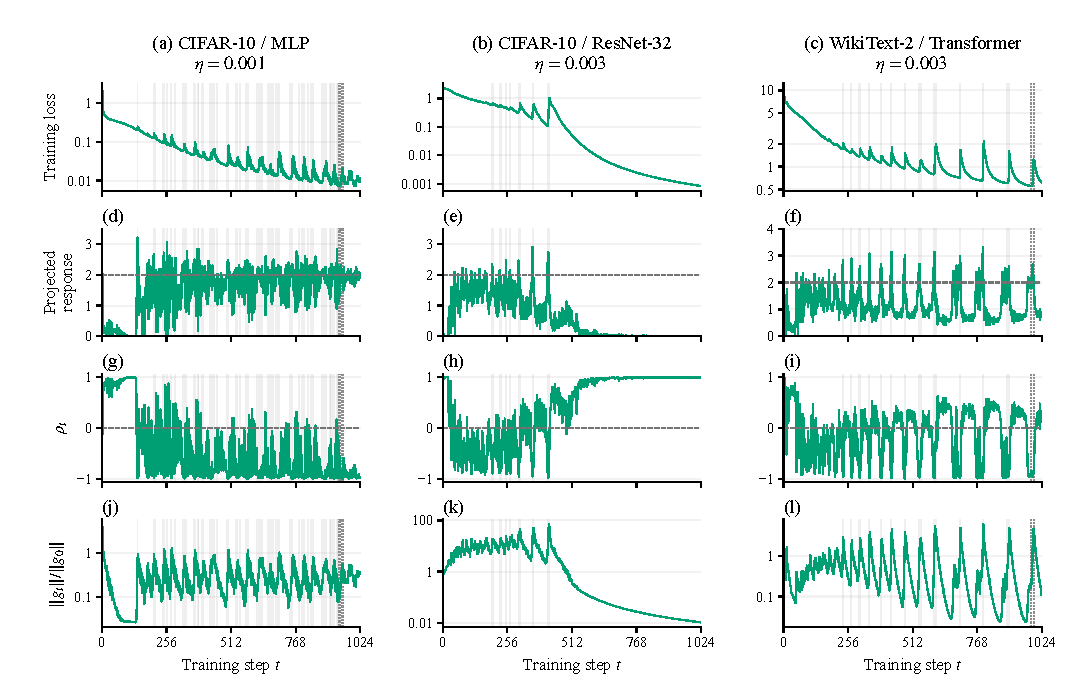
\includegraphics[width=\textwidth]{figures/00-high-lr-overview-cifar10-mlp-resnet-wikitext2-transformer.pdf}
\caption{Loss spikes and consecutive-gradient behavior under full-objective Adam. Columns are MLP, ResNet-32, and Transformer, at learning rates $.001/.003/.003$. Rows show loss, the projected gradient response $1-\rho_t\|g_t\|/\|g_{t-1}\|$, consecutive-gradient cosine, and gradient norm relative to initialization.}
\label{fig:adam-overview}
\end{figure*}

Adam exhibits markedly different dynamics from full-batch GD. While GD remains in the destructive regime despite a sustained overall loss decrease (Section~\ref{sec:gd-experiments}), Adam undergoes recurrent loss spikes that begin with negative alignment ($\rho_t<0$) and increasing gradient norms (Fig.~\ref{fig:adam-overview}). During recovery, it can move to constructive regime ($\rho_t>0$), while gradient norms and loss decline. In most cases, the loss eventually falls below its pre-spike value. From an optimization perspective, these excursions may allow Adam to traverse higher-loss regions and reach lower-loss basins. It suggests that suppressing spikes by reducing the learning rate could also lead to premature convergence. 

We then ask whether raw gradients can predict a loss increase before Adam applies the next update. For quadratic full-batch GD, Eq.~\eqref{eq:loss-rise-alignment} shows that the preceding step raises the loss exactly when $\eta\widehat{\kappa}_t=1-\rho_t\|g_t\|/\|g_{t-1}\|>2$. Under Adam, we test whether this raw-gradient condition predicts a loss increase of at least 0.1\% on the next step, $(L_{t+1}-L_t)/L_t\geq0.001$, where $L_t=\mathcal L(\theta_t)$. Table~\ref{tab:severity} compares the combined condition with constant predictions, the preceding loss change ($L_t>L_{t-1}$), and rules based on alignment or norm growth alone. Across all three models, the combined condition achieves the highest accuracy and warning lift.

\begin{table*}[!t]
\centering\small
\caption{Prediction of a loss increase of at least 0.1\% on the next Adam step. Acc. is accuracy. Hit is the percentage of warnings followed by such an increase (precision). Lift is precision divided by the baseline event rate.}
\label{tab:severity}
\setlength{\tabcolsep}{4pt}
\begin{tabular}{@{}lrrrrrrrrr@{}}
\toprule
& \multicolumn{3}{c}{MLP} & \multicolumn{3}{c}{ResNet} & \multicolumn{3}{c}{Transformer} \\
Condition & Acc. (\%) & Hit (\%) & Lift ($\times$) & Acc. (\%) & Hit (\%) & Lift ($\times$) & Acc. (\%) & Hit (\%) & Lift ($\times$) \\
\midrule
Baseline event rate & \multicolumn{3}{c}{446/1023 (43.6\%)} & \multicolumn{3}{c}{88/1023 (8.6\%)} & \multicolumn{3}{c}{142/1023 (13.9\%)} \\
\midrule
Always predict no increase & 56.4 & -- & -- & 91.4 & -- & -- & 86.1 & -- & -- \\
Always predict increase & 43.6 & 43.6 & 1.00 & 8.6 & 8.6 & 1.00 & 13.9 & 13.9 & 1.00 \\
$L_t>L_{t-1}$ & 58.1 & 51.9 & 1.19 & 89.0 & 36.8 & 4.28 & 86.5 & 51.3 & 3.70 \\
$\rho_t<0$ & 54.4 & 48.8 & 1.12 & 77.9 & 27.0 & 3.14 & 61.6 & 25.9 & 1.87 \\
$\|g_t\|>\|g_{t-1}\|$ & 53.5 & 47.3 & 1.08 & 68.7 & 14.2 & 1.65 & 63.1 & 22.1 & 1.59 \\
$\rho_t<-\|g_{t-1}\|/\|g_t\|$ & 59.9 & 55.8 & 1.28 & 92.0 & 58.3 & 6.78 & 87.2 & 53.7 & 3.87 \\
\bottomrule
\end{tabular}
\end{table*}



\subsection{Tracing Oscillations through the Learned Function}
\label{subsec:tracing}

\begin{figure*}[!t]
\centering
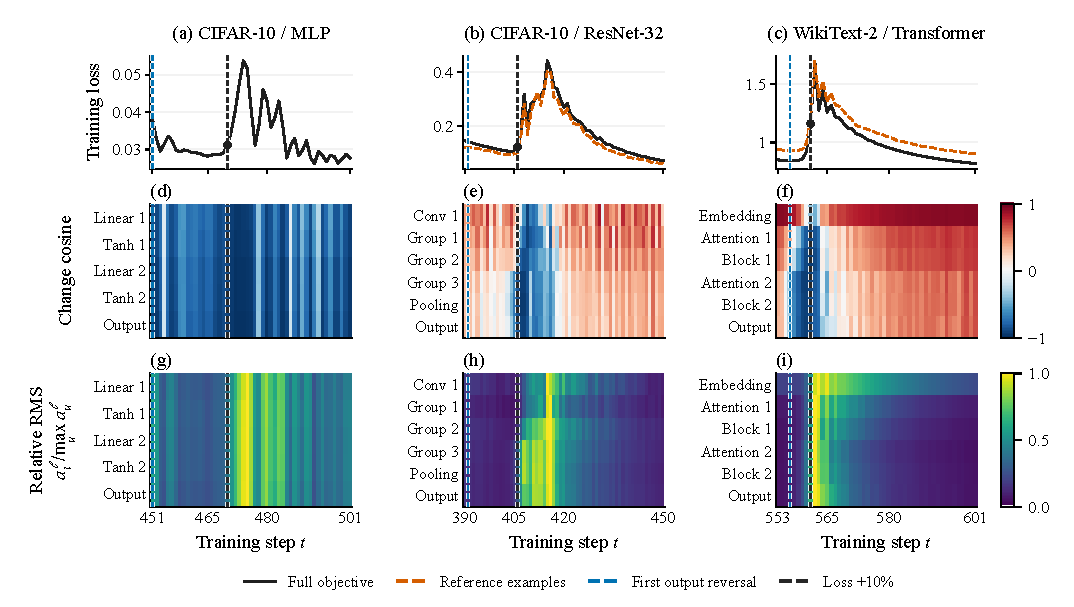
\includegraphics[width=\textwidth]{figures/00-three-model-loss-representation-motion.pdf}
\caption{Loss and representation changes during selected Adam spikes in the MLP (steps 451--501), ResNet (390--450), and Transformer (553--601). Top: training loss and loss on fixed reference inputs. Middle: cosine between consecutive representation changes at each measured site (blue: reversal; red: reinforcement). Bottom: RMS displacement normalized by each site's maximum within the window. Blue dashed lines mark the first displayed negative output-change cosine (already negative for the MLP); black dashed lines mark when loss first exceeds the pre-peak minimum by 10\%.}
\label{fig:trace-motion}
\end{figure*}

To examine how constructive and destructive gradient regimes manifest in the network's functional behavior, we track changes in hidden representations and outputs induced by each Adam update on a fixed set of inputs. We use all 5,000 training images for the MLP, the first intact 1,000-image BatchNorm group for ResNet, and the first 64 complete sequences (2,240 token positions) for the Transformer. At each measured site $\ell$ (a selected layer, attention module, residual block group, or network output), let $A_t^\ell\in\mathbb{R}^{N_\ell\times m_\ell}$ denote the responses after $t$ updates, with rows corresponding to fixed inputs or token positions and columns to features. The $t$th update induces the representation change
\begin{equation}
 \delta_t^\ell=\operatorname{vec}(A_t^\ell-A_{t-1}^\ell)
 \in\mathbb R^{P_\ell},\qquad P_\ell=N_\ell m_\ell.
 \label{eq:representation-change}
\end{equation}
At site $\ell$, we measure the alignment between consecutive representation changes by their cosine $c_t^\ell$ and the size of each change by its root-mean-square displacement $a_t^\ell$
\begin{equation}
 c_t^\ell=
 \frac{\langle\delta_{t-1}^\ell,\delta_t^\ell\rangle}
 {\|\delta_{t-1}^\ell\|\|\delta_t^\ell\|},\qquad
 a_t^\ell=\frac{\|\delta_t^\ell\|}{\sqrt{P_\ell}}.
 \label{eq:representation-motion}
\end{equation}
Like $\rho_t$ for gradients, $c_t^\ell$ distinguishes constructive ($c_t^\ell>0$) from destructive ($c_t^\ell<0$) alignment, here over all measured responses at the site. To quantify how these changes accumulate over updates $t=a,\ldots,b$, we define displacement retention $R_{a:b}^\ell$ as the ratio of net displacement to total distance traveled
\begin{equation}
 R_{a:b}^\ell=
 \frac{\|\sum_{t=a}^b\delta_t^\ell\|}{\sum_{t=a}^b\|\delta_t^\ell\|}
 =\frac{\|A_b^\ell-A_{a-1}^\ell\|_{\mathrm{F}}}
 {\sum_{t=a}^b\|A_t^\ell-A_{t-1}^\ell\|_{\mathrm{F}}}.
 \label{eq:representation-retention}
\end{equation}
Here $\|M\|_{\mathrm{F}}=(\sum_{i,j}M_{ij}^2)^{1/2}$ denotes the Frobenius norm, i.e. the Euclidean norm of the vector obtained by flattening $M$.

Figure~\ref{fig:trace-motion} traces representation changes during one selected loss spike per model. Output changes become negatively aligned before the sharp loss increase in ResNet and the Transformer, while the MLP is already in the destructive regime at the start of the window. Across all three models, representation changes are largest near the loss peak, but their alignment differs across depth: outputs can exhibit destructive reversals even while earlier layers remain constructive. These oscillations produce substantial cancellation, with only 1.71\%, 2.44\%, and 3.51\% of the total output path retained in the MLP, ResNet, and Transformer, respectively. While retention is also low in the earliest measured layers of the MLP and ResNet (3.25\% and 3.72\%), the Transformer's embedding retains 24.33\%, indicating that large output oscillations can coexist with more persistent changes in earlier representations.

Do successive updates repeatedly reverse the same patterns of change in the network's representations? To investigate this, we stack the representation changes $(\delta_t^\ell)^\top$ over each spike window $t=a,\ldots,b$ into a matrix $D_\ell$ and compute its singular value decomposition (SVD),
\begin{equation}
 D_\ell=U_\ell\Sigma_\ell V_\ell^\top.
 \label{eq:temporal-svd}
\end{equation}
Each right singular vector $v_{\ell,j}$ defines a fixed pattern of change across reference inputs and features. We project each update onto these directions,
\begin{equation}
 \alpha_{t,j}^\ell=\langle\delta_t^\ell,v_{\ell,j}\rangle,\qquad
 \delta_t^\ell=\sum_j\alpha_{t,j}^\ell v_{\ell,j}.
 \label{eq:pattern-reconstruction}
\end{equation}
A change in the sign of $\alpha_{t,j}^\ell$ indicates a reversal along the same pattern. To measure how concentrated these changes are, we compute the fraction of total squared movement captured by the first $k$ directions,
\begin{equation}
 E_k^\ell=\frac{\sum_{j=1}^k\sigma_{\ell,j}^2}
 {\sum_j\sigma_{\ell,j}^2},
 \label{eq:energy}
\end{equation}
where the singular values $\sigma_{\ell,j}$ are ordered from largest to smallest.

\begin{figure*}[!t]
\centering
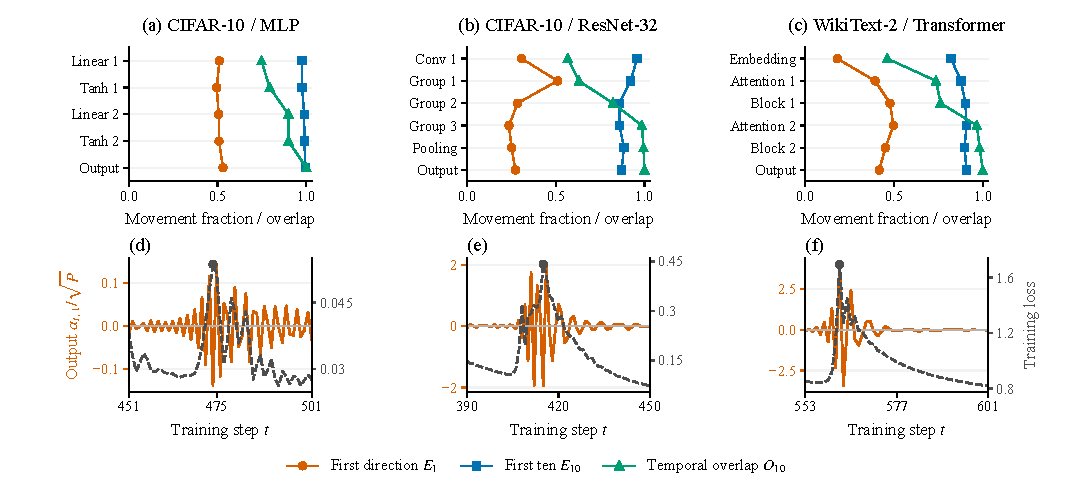
\includegraphics[width=\textwidth]{figures/01-three-model-temporal-structure.pdf}
\caption{Concentration and reversal of representation changes during the spike windows in Fig.~\ref{fig:trace-motion} (51 updates for the MLP, 61 for ResNet, and 49 for the Transformer). (a)--(c) At each site, orange circles and blue squares show the fractions of squared movement captured by the first direction ($E_1$) and the first ten directions ($E_{10}$). Green triangles show the temporal overlap ($O_{10}$) between the leading ten directions at that site and at the output. (d)--(f) The orange curve shows signed displacement per update along the leading output direction summarized by the orange output marker above (left axis). Each sign change marks a reversal. The dashed gray curve shows training loss (right axis), with a dot at its peak.}
\label{fig:trace-structure}
\end{figure*}

To compare the temporal structure of representation changes across sites, we use the left singular vectors $U_\ell$. Each column describes how a dominant pattern of change varies in magnitude and direction across successive updates. Let $U_{\ell,k}$ contain the first $k$ columns of $U_\ell$. We define their temporal overlap with the output as
\begin{equation}
 O_k(\ell,\mathrm{out})=\frac{\|U_{\ell,k}^\top U_{\mathrm{out},k}\|_{\mathrm{F}}^2}{k},
 \label{eq:overlap}
\end{equation}
where an overlap of one indicates identical temporal subspaces.

Figure~\ref{fig:trace-structure} shows that representation changes during loss spikes are highly concentrated in a few directions. Across all models and measured sites, the first ten directions capture 82--99\% of total squared movement. At the output, the leading direction alone accounts for 53\%, 27\%, and 42\% in the MLP, ResNet, and Transformer, respectively. Importantly, updates repeatedly reverse along this same direction over the spike windows (Fig.~\ref{fig:trace-structure}d--f). These oscillations also exhibit shared temporal structure across network depth. In ResNet, the overlap $O_{10}$ with the output increases from 0.57 at the first convolution to 0.99 at the final residual stage. Similarly, in the Transformer, it increases from 0.46 at the embedding to 0.98 at the final block. Together, these findings reveal that loss spikes involve a structured, low-dimensional oscillations shared accross the network sites that repeatedly reverse functional changes. It then motivates an intervention that limits large representation changes.

